% Intestazione
\fancyhead[L]{3 \hspace{0.2cm} Casi d'uso} % Testo a sinistra

\section{Casi d'uso}
\label{sec:casi_uso}

\subsection{Scopo}

Lo scopo di questa sezione è descrivere in maniera dettagliata i casi d’uso individuati dal
gruppo, in riferimento alle funzionalità dell’applicazione.


\subsection{Attori}

L’applicazione prevede la presenza di \dots


\subsection{Lista casi d'uso}



\hypertarget{UC5}{}
\subsubsection{UC5: Visualizzazione della risposta generata}

\begin{figure}[h]
    \centering
    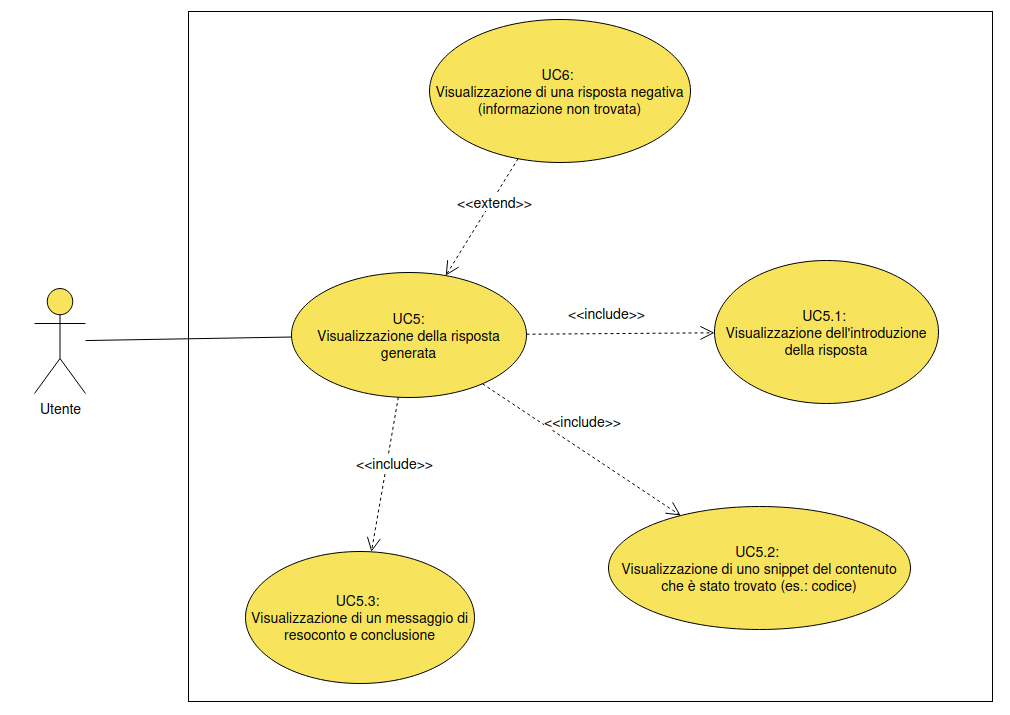
\includegraphics[width=\textwidth]{Diagramma UC5 - Visualizzazione della risposta generata.png}
    \caption{Visualizzazione della risposta generata}
\end{figure}

\begin{itemize}
    \item \textbf{Attori coinvolti}: Utente
    \item \textbf{Precondizioni}: BuddyBot ha generato correttamente la risposta alla domanda dell'utente.
    \item \textbf{Postcondizioni}: L'utente visualizza la risposta generata da BuddyBot
    \item \textbf{\emph{Scenario principale}\textsubscript{\textbf{\textit{G}}}}:
    \begin{enumerate}
        \item BuddyBot ha generato correttamente la risposta alla domanda dell'utente;
        \item L'utente visualizza la risposta generata da BuddyBot.
    \end{enumerate}
    \item \textbf{Sottocasi d'uso}:
    \begin{itemize}
        \item \textbf{UC5.1}: Visualizzazione dell'introduzione della risposta;
        \item \textbf{UC5.2}: Visualizzazione di uno snippet del contenuto che è stato trovato (es.: codice);
        \item \textbf{UC5.3}: Visualizzazione di un messaggio di resoconto e conclusione.
    \end{itemize}
\end{itemize}



\subsubsubsection{UC5.1: Visualizzazione dell'introduzione della risposta}

\begin{itemize}
    \item \textbf{Attori coinvolti}: Utente
    \item \textbf{Precondizioni}: BuddyBot ha generato correttamente la risposta alla domanda dell'utente.
    \item \textbf{Postcondizioni}: L'utente visualizza l'introduzione della risposta generata da BuddyBot.
    \item \textbf{\emph{Scenario principale}\textsubscript{\textbf{\textit{G}}}}:
    \begin{enumerate}
        \item BuddyBot ha generato correttamente la risposta alla domanda dell'utente;
        \item L'utente visualizza l'introduzione della risposta generata da BuddyBot.
    \end{enumerate}
\end{itemize}



\subsubsubsection{UC5.2: Visualizzazione di uno snippet del contenuto che è stato trovato (es.: codice)}

\begin{itemize}
    \item \textbf{Attori coinvolti}: Utente
    \item \textbf{Precondizioni}: 
    \begin{itemize}
        \item L'utente ha visualizzato l'introduzione della risposta generata da BuddyBot.
        \item La risposta generata da BuddyBot contiene uno snippet di codice.
    \end{itemize}
    \item \textbf{Postcondizioni}: L'utente visualizza uno snippet di codice contenuto della risposta generata da BuddyBot.
    \item \textbf{\emph{Scenario principale}\textsubscript{\textbf{\textit{G}}}}:
    \begin{enumerate}
        \item L'utente ha visualizzato l'introduzione della risposta generata da BuddyBot;
        \item L'utente visualizza uno snippet del contenuto che è stato trovato (es.: codice).
    \end{enumerate}
\end{itemize}



\subsubsubsection{UC5.3: Visualizzazione di un messaggio di resoconto e conclusione}

\begin{itemize}
    \item \textbf{Attori coinvolti}: Utente
    \item \textbf{Precondizioni}: L'utente ha visualizzato almeno l'introduzione della risposta generata da BuddyBot.
    \item \textbf{Postcondizioni}: L'utente visualizza un messaggio di resoconto e conclusione contenuto nella risposta generata da BuddyBot.
    \item \textbf{\emph{Scenario principale}\textsubscript{\textbf{\textit{G}}}}:
    \begin{enumerate}
        \item L'utente ha visualizzato l'introduzione della risposta generata da BuddyBot, e, se presente, uno snippet di codice in essa contenuto;
        \item L'utente visualizza un messaggio di resoconto e conclusione che termina la risposta.
    \end{enumerate}
\end{itemize}



\hypertarget{UC6}{}
\subsubsection{UC6: Visualizzazione di una risposta negativa (informazione non trovata)}

\begin{itemize}
    \item \textbf{Attori coinvolti}: Utente
    \item \textbf{Precondizioni}: BuddyBot non ha trovato l'informazione che l'utente ha domandato.
    \item \textbf{Postcondizioni}: L'utente visualizza come risposta un messaggio di BuddyBot in cui gli viene segnalata la mancanza dell'informazione 
    richiesta nei dati forniti come contesto.
    \item \textbf{\emph{Scenario principale}\textsubscript{\textbf{\textit{G}}}}:
    \begin{enumerate}
        \item BuddyBot non ha trovato l'informazione che l'utente ha domandato;
        \item L'utente visualizza come risposta un messaggio di BuddyBot in cui gli viene segnalata la mancanza dell'informazione richiesta 
        nei dati forniti come contesto.
    \end{enumerate}
\end{itemize}







\hypertarget{UC11}{}
\subsubsection{UC11: Aggiornamento automatico del database vettoriale}

\begin{figure}[h]
    \centering
    
\includegraphics[width=\textwidth]{placeholder.png}
    \caption{Aggiornamento automatico del database vettoriale}
\end{figure}

\begin{itemize}
    \item \textbf{Attori coinvolti}: BuddyBot, \emph{GitHub}\textsubscript{\textbf{\textit{G}}}, \emph{Jira}\textsubscript{\textbf{\textit{G}}}, 
    \emph{Confluence}\textsubscript{\textbf{\textit{G}}}, \emph{Modello di Embedding}\textsubscript{\textbf{\textit{G}}}, 
    \emph{Database vettoriale}\textsubscript{\textbf{\textit{G}}}
    \item \textbf{Precondizioni}: 
    \begin{itemize}
        \item È giunto il momento periodico in cui aggiornare il database vettoriale;
        \item È possibile collegarsi tramite \emph{API}\textsubscript{\textbf{\textit{G}}} a GitHub, Jira, Confluence ed al Modello di Embedding.
        \item Il database vettoriale è stato avviato.
    \end{itemize}
    \item \textbf{Postcondizioni}: Il database vettoriale è aggiornato con le informazioni più recenti disponibili in GitHub, Jira e Confluence.
    \item \textbf{\emph{Scenario principale}\textsubscript{\textbf{\textit{G}}}}:
    \begin{enumerate}
        \item BuddyBot, periodicamente, si collega a GitHub, Jira e Confluence per ottenere eventuali aggiornamenti;
        \item Se ci sono aggiornamenti, BuddyBot si collega al Modello di Embedding per convertire le informazioni ottenute in formato vettoriale;
        \item BuddyBot aggiorna il database vettoriale con le informazioni ottenute;
        \item Nel caso in cui l'aggiornamento del database vettoriale è fallito, cioè quando sono stati rilevati nuovi dati ma non è stato possibile 
        farne il retrieval, alle successive domande dell'utente il bot fornisce le risposte normalmente, ma segnalando che queste ultime potrebbero 
        essere basate su dati obsoleti.
    \end{enumerate}
    \item \textbf{Sottocasi d'uso}:
    \begin{itemize}
        \item \textbf{UC11.1}: Chiamata API verso GitHub per il retrieval di eventuali nuove modifiche;
        \item \textbf{UC11.2}: Chiamata API verso Jira per il retrieval di eventuali nuove modifiche;
        \item \textbf{UC11.3}: Chiamata API verso Confluence per il retrieval di eventuali nuove modifiche;
        \item \textbf{UC11.4}: Merge dei nuovi dati con i dati già presenti nel database vettoriale.
    \end{itemize}
\end{itemize}



\subsubsubsection{UC11.1: Chiamata API verso GitHub per il retrieval di eventuali nuove modifiche}

\begin{itemize}
    \item \textbf{Attori coinvolti}: BuddyBot, \emph{GitHub}\textsubscript{\textbf{\textit{G}}}
    \item \textbf{Precondizioni}: 
    \begin{itemize}
        \item È giunto il momento periodico in cui aggiornare il database vettoriale;
        \item È possibile collegarsi tramite \emph{API}\textsubscript{\textbf{\textit{G}}} a GitHub.
    \end{itemize}
    \item \textbf{Postcondizioni}: Vengono restituiti gli aggiornamenti che sono avvenuti su GitHub rispetto all'ultima richiesta, eventualmente nessuno 
    se GitHub non è stato aggiornato.
    \item \textbf{\emph{Scenario principale}\textsubscript{\textbf{\textit{G}}}}: BuddyBot, periodicamente, si collega a GitHub per ottenere eventuali aggiornamenti.
\end{itemize}



\subsubsubsection{UC11.2: Chiamata API verso Jira per il retrieval di eventuali nuove modifiche}

\begin{itemize}
    \item \textbf{Attori coinvolti}: BuddyBot, \emph{Jira}\textsubscript{\textbf{\textit{G}}}
    \item \textbf{Precondizioni}:
    \begin{itemize}
        \item È giunto il momento periodico in cui aggiornare il database vettoriale;
        \item È possibile collegarsi tramite \emph{API}\textsubscript{\textbf{\textit{G}}} a Jira.
    \end{itemize}
    \item \textbf{Postcondizioni}: Vengono restituiti gli aggiornamenti che sono avvenuti su Jira rispetto all'ultima richiesta, eventualmente nessuno 
    se Jira non è stato aggiornato.
    \item \textbf{\emph{Scenario principale}\textsubscript{\textbf{\textit{G}}}}: BuddyBot, periodicamente, si collega a Jira per ottenere eventuali aggiornamenti.
\end{itemize}



\subsubsubsection{UC11.3: Chiamata API verso Confluence per il retrieval di eventuali nuove modifiche}

\begin{itemize}
    \item \textbf{Attori coinvolti}: BuddyBot, \emph{Confluence}\textsubscript{\textbf{\textit{G}}}
    \item \textbf{Precondizioni}: 
    \begin{itemize}
        \item È giunto il momento periodico in cui aggiornare il database vettoriale;
        \item È possibile collegarsi tramite \emph{API}\textsubscript{\textbf{\textit{G}}} a Confluence.
    \end{itemize}
    \item \textbf{Postcondizioni}: Vengono restituiti gli aggiornamenti che sono avvenuti su Confluence rispetto all'ultima richiesta, eventualmente nessuno 
    se Confkuence non è stato aggiornato.
    \item \textbf{\emph{Scenario principale}\textsubscript{\textbf{\textit{G}}}}: BuddyBot, periodicamente, si collega a Confluence per ottenere eventuali aggiornamenti.
\end{itemize}



\subsubsubsection{UC11.4: Merge dei nuovi dati con i dati già presenti nel database vettoriale}

\begin{itemize}
    \item \textbf{Attori coinvolti}: BuddyBot, \emph{Modello di Embedding}\textsubscript{\textbf{\textit{G}}}, 
    \emph{Database vettoriale}\textsubscript{\textbf{\textit{G}}}
    \item \textbf{Precondizioni}: 
    \begin{itemize}
        \item BuddyBot ha ottenuto nuovi dati da GitHub, Jira e Confluence;
        \item È possibile collegarsi tramite \emph{API}\textsubscript{\textbf{\textit{G}}} al Modello di Embedding;
        \item Il database vettoriale è stato avviato.
    \end{itemize}
    \item \textbf{Postcondizioni}: Il database vettoriale è aggiornato con le informazioni più recenti disponibili in GitHub, Jira e Confluence.
    \item \textbf{\emph{Scenario principale}\textsubscript{\textbf{\textit{G}}}}:
    \begin{enumerate}
        \item Se ci sono aggiornamenti su GitHub, Jira o Confluence, BuddyBot si collega al Modello di Embedding per convertire le informazioni 
        ottenute in formato vettoriale;
        \item BuddyBot aggiorna il database vettoriale con le informazioni ottenute;
    \end{enumerate}
    \item \textbf{Sottocasi d'uso}:
    \begin{itemize}
        \item \textbf{UC11.4.1}: Conversione dei nuovi dati in formato vettoriale.
    \end{itemize}
\end{itemize}



\paragraph{UC11.4.1: Conversione dei nuovi dati in formato vettoriale}

\begin{itemize}
    \item \textbf{Attori coinvolti}: BuddyBot, \emph{Modello di Embedding}\textsubscript{\textbf{\textit{G}}}
    \item \textbf{Precondizioni}: 
    \begin{itemize}
        \item BuddyBot ha ottenuto nuovi dati da GitHub, Jira e Confluence;
        \item È possibile collegarsi tramite \emph{API}\textsubscript{\textbf{\textit{G}}} al Modello di Embedding;
    \end{itemize}
    \item \textbf{Postcondizioni}: Le informazioni più recenti disponibili in GitHub, Jira e Confluence sono state convertite in formato vettoriale.
    \item \textbf{\emph{Scenario principale}\textsubscript{\textbf{\textit{G}}}}: Se ci sono aggiornamenti su GitHub, Jira o Confluence, BuddyBot si collega al Modello di Embedding per convertire le informazioni 
        ottenute in formato vettoriale.
\end{itemize}



\hypertarget{UC15}{}
\subsubsection{UC15: Visualizzazione della frase "la risposta è basata su dati che potrebbero essere obsoleti" sopra alle successive risposte del chatbot}

\begin{itemize}
    \item \textbf{Attori coinvolti}: BuddyBot, Utente
    \item \textbf{Precondizioni}: L'utente ha posto una domanda a BuddyBot
    \item \textbf{Postcondizioni}: L'utente, oltre alla consueta risposta del chatbot, visualizza sopra di essa una frase che lo avvisa del fatto che i dati usati per 
    costruire la risposta sono obsoleti.
    \item \textbf{\emph{Scenario principale}\textsubscript{\textbf{\textit{G}}}}:
    \begin{enumerate}
        \item Utente pone una domanda a BuddyBot;
        \item BuddyBot risponde alla domanda dell'utente;
        \item L'utente visualizza la risposta del chatbot anticipata dalla frase "la risposta è basata su dati che potrebbero essere obsoleti".
    \end{enumerate}
\end{itemize}